\documentclass[11pt]{article}

\usepackage[margin=1in]{geometry}
\usepackage{amsmath,amssymb}
\usepackage{booktabs}
\usepackage{graphicx}
\usepackage{xcolor}
\usepackage[colorlinks=true,linkcolor=linkblue,citecolor=linkblue,urlcolor=linkblue]{hyperref}
\usepackage{url}
\usepackage{algorithm}
\usepackage{algpseudocode}
\usepackage{caption}
\usepackage{subcaption}
\usepackage{microtype}
\usepackage{enumitem}

\definecolor{linkblue}{RGB}{0,80,160}

\newcommand{\choice}{\texttt{choice}}
\newcommand{\score}{\texttt{score}}
\newcommand{\noul}{\texttt{noul}}
\newcommand{\openjev}{OpenJev}

\title{\textbf{\openjev{}: Typed Decisions from Small Models}\\[0.35em]
\large What it takes to make a 150M encoder, or a 1.7B decoder,\\
answer many typed questions about one input in a single forward pass}

\author{%
  Prathamesh Saraf \\
  \texttt{\href{https://github.com/S1LV3RJ1NX/openjev}{github.com/S1LV3RJ1NX/openjev}}
}

\date{September 2026}

\begin{document}
\maketitle

\begin{abstract}
A large class of production decisions is not open-ended generation but a
fixed menu: route this message to one of 77 intents, flag whether it
mentions clinical risk, rate its urgency on a four-point scale. Language
models answer such questions by generating text that must then be parsed
and constrained, at a cost per question and with no guarantee the answer
lies on the menu.

We describe \openjev{}, an open architecture for \emph{typed decisions}. A
state is encoded once as a shared prefix; every candidate option is placed
after it behind a marker token; block-diagonal attention isolates the
questions from one another; and a grouped log-softmax normalises scores
within each question's own option set. Ten questions about one input
therefore cost one forward pass, and the answer is a calibrated probability
over a closed menu rather than generated text. Latency is flat in the
number of questions: ten cost 6\% more than one.

Our central finding is that this architecture, on its own, does not
generalize. A strong bidirectional encoder with the output format and no
task training scores \textbf{0.7$\times$ chance} on held-out schemas, and a
61-task training mixture leaves it at 0.9$\times$. Generalization comes from
the composition of the training data, and specifically from properties that
are cheap to synthesize: padding training menus with borrowed distractor
labels takes accuracy on a 77-way held-out menu from a literal $0.000$ to
$0.205$, because a model that has never seen a large menu collapses onto one
label when handed one. Scaling an audited mixture to 279 tasks and 323{,}466
rows brings the held-out suite to \textbf{21.9$\times$ chance}, with all
seven tasks clearing their chance floor and a 151-way menu reaching
94.9$\times$.

Given labels for the target task, small models are competitive with a
commercial typed-decision API. A rank-16 LoRA adapter on Qwen3-1.7B, trained
on 395 examples in 258 seconds, \textbf{beats} that API on a healthcare
routing benchmark: intent $0.979$ against $0.941$ ($p=1\mathrm{e}{-3}$),
multi-label exact set $0.909$ against $0.822$ ($p=7\mathrm{e}{-6}$), and
three simultaneous intents $0.903$ against $0.645$; three wins, four
statistical ties, no losses. Notably the adapter, at $17$M trainable
parameters and $87$\,MB, outperforms opening all $1{,}725$M ($0.929$,
$3.4$\,GB).

We also report where this fails. Without labels the gap remains large:
$0.290$ on Banking77 against roughly $0.820$. And benchmark transfer is not
deployment readiness. The same general checkpoint scoring 21.9$\times$
chance, applied zero-shot to the routing task, reaches intent $0.601$ and a
clinical-gate recall of $0.111$. Every claim here is reproducible from a
public repository, with datasets, checkpoints, and the negative results
reported alongside the positive ones.

\end{abstract}

\section{Introduction}
\label{sec:intro}

Consider a pharmacy support queue. A message arrives: \emph{``I need a
refill on my thyroid tablets, and are you open on Sunday? Also I've been
getting dizzy since starting them.''} A system routing this must decide,
simultaneously, which topics it concerns (two), whether it mentions
clinical risk that a human should see (it does), and how urgent it is.
Each of these is a decision over a \emph{known, closed} set of answers.

The dominant approach is to ask a language model and parse what comes back.
This works, and it is expensive in three distinct ways. Each question costs
its own generation. The output is unconstrained, so it must be coerced onto
the menu by grammar-constrained decoding or by retrying. And the resulting
token probabilities are a poor basis for the thresholding that operational
systems need, because they describe a sampling distribution over strings
rather than a calibrated belief over options.

\subsection{Typed decisions}

We use \emph{typed decision} for a question whose answer set is fixed in
advance and known to the system. Three types cover most of what production
routing and guardrail systems need:

\begin{itemize}[leftmargin=1.4em,itemsep=0.25em]
  \item \choice{} --- exactly one of $K$ options. Intent, category, routing
    target. $K$ reaches 151 in our evaluation.
  \item \score{} --- one level on an \emph{ordered} scale. Severity,
    urgency, quality. The ordering is information a \choice{} discards.
  \item \noul{} --- yes or no. Flags and safety gates. Several asked
    together express multi-label structure, which a single \choice{}
    cannot: a softmax over intents has no way to say ``both''.
\end{itemize}

\subsection{What this paper is about}

\openjev{} is an open implementation of an architecture for answering many
such questions about one input at once, and an empirical account of what
makes it work. We set out to reproduce the behaviour of a commercial
typed-decision API, and the interesting result is not the architecture,
which is a recombination of published ideas (\S\ref{sec:background}). It is
which parts of the recipe actually carry the performance.

Three findings organise the paper.

\paragraph{The architecture does not generalize on its own.} A pretrained
bidirectional encoder, given the option-scoring output format and no task
training, scores $0.7\times$ chance on held-out schemas --- worse than
guessing. Its larger sibling reaches $2.2\times$. The output format makes
zero-shot scoring \emph{possible}; it does not make it \emph{present}
(\S\ref{sec:res-architecture}).

\paragraph{Generalization is a property of the training mixture, and some
of it is synthesizable.} Our first mixture left held-out transfer at
$0.9\times$ chance. The single largest fix was not more data but a
different \emph{shape} of data: padding training menus with distractor
labels borrowed from other tasks, which moved a 77-way held-out menu from a
literal $0.000$ to $0.205$. A model that has never seen a large menu
collapses onto one label when handed one, and you can manufacture large
menus without finding datasets that have them (\S\ref{sec:res-data}).

\paragraph{With labels, small models win; without them, they do not.} A
rank-16 adapter on a 1.7B backbone, trained on 395 examples, beats the
commercial API on three of seven router measures and ties the rest. The
same architecture without task labels remains far behind it. That split is
the honest summary of where this technology stands
(\S\ref{sec:res-router}, \S\ref{sec:discussion}).

\subsection{Contributions}

\begin{enumerate}[leftmargin=1.5em,itemsep=0.25em]
  \item An architecture and open implementation for multi-question typed
    decisions in a single forward pass, with latency flat in the number of
    questions (10 questions cost 6\% more than 1) and full-precision
    calibrated probabilities.
  \item \emph{Label-space augmentation}, a training-time intervention that
    manufactures the menu-size diversity a mixture lacks, and which is the
    difference between no transfer and useful transfer at high cardinality.
  \item A measured account of parameter-efficient fine-tuning for this task
    shape, including the result that a 17M-parameter adapter outperforms
    opening all 1{,}725M parameters, at $1/39$ the artifact size.
  \item A reproducible benchmark suite with an enforced contamination
    guard, a held-in control that distinguishes ``no transfer'' from ``a
    bug'', and a hardened routing task built to retain headroom where the
    reference system saturated.
  \item A set of negative and retracted results reported at the same
    prominence as the positive ones (\S\ref{sec:ablations}), including two
    interventions that made things worse and one conclusion we withdrew
    after finding the bug that produced it.
\end{enumerate}

Everything is reproducible from a public repository, with released
checkpoints, adapters, and datasets listed in Appendix~\ref{app:artifacts}.

\section{Background and related work}
\label{sec:background}

Every structural idea in \openjev{} exists in the literature. We state the
provenance plainly, because the paper's contribution is empirical rather
than architectural.

\paragraph{Scoring options instead of generating them.}
UniMC~\cite{unimc} recasts multiple-choice NLU by inserting an
option-marker token before each candidate and reading a decision from the
encoder's state at that position, avoiding generation entirely. Our readout
is the same idea. The consequence people usually reach for, that such a
model ``cannot hallucinate'', is narrower than it sounds: the model
cannot emit a string outside the menu, which says nothing about whether the
option it picks is right.

\paragraph{Encoding a shared prefix once.}
Parallel Context Windows~\cite{pcw} and related work formalise attention
masks in which several segments each attend to a common prefix and to
themselves, but not to one another. We use exactly this to isolate
questions, so that an answer does not depend on which other questions were
asked in the same call. On a causal backbone the prefix is ordinary
left-context, which is what a KV cache is for.

\paragraph{Multi-task training for zero-shot transfer.}
T0~\cite{t0} and the Flan collection~\cite{flan} establish that training
across many tasks produces zero-shot ability on unseen ones, and that the
gain continues accruing with task count into the high hundreds. Our mixture
is assembled from \texttt{tasksource}~\cite{tasksource}, which normalises a
large number of classification and multiple-choice datasets into a common
interface. Flan's task-count finding is the reason we treat 279 tasks as a
floor rather than a target.

\paragraph{Intermediate-task transfer.}
Training on an intermediate task before the target is
STILTs~\cite{stilts}; the domain-adaptive variant is
Gururangan et al.~\cite{dontstoppretraining}. Both report that the gain is largest when the
target dataset is small, and that it is inconsistent across task pairs and
can be negative. We observe both effects: a large gain at 395 target
examples (\S\ref{sec:res-router}), and two mixture changes that made
held-out transfer \emph{worse} (\S\ref{sec:ablations}).

\paragraph{Parameter-efficient adaptation.}
LoRA~\cite{lora} trains low-rank updates beside frozen weights. Our use is
conventional; the finding that it \emph{outperforms} full fine-tuning here,
rather than merely approximating it cheaply, is reported in
\S\ref{sec:res-router} together with the most likely explanation.

\paragraph{Ordinal and rejection heads.}
CORN/CORAL~\cite{corn} give rank-consistent ordinal objectives, and
adaptive decision boundaries~\cite{adb} detect out-of-scope inputs without
negative samples. We implement neither; \score{} is currently a softmax
over levels whose order is used only in rendering and in the
expectation-based readout. This is a limitation and we mark it as such
(\S\ref{sec:discussion}).

\paragraph{The system we compare against.}
Our reference is a commercial typed-decision API, \texttt{jev-1.13.0} from
TypeSafe, measured by black-box probing on 20 September 2026 at the sample
sizes stated. We inferred its design from behaviour: latency is flat from 2
to 255 options and an eight-question call costs the same wall time as a
one-question call, which is the signature of a shared prefix with parallel
readout. All figures attributed to it are one-day measurements of a hosted
endpoint from one network location, and should be reproduced before being
relied on.

Laya, from Convai Innovations, is the closest open-source system: the
same three primitives behind a near-identical
interface.\footnote{\url{https://huggingface.co/convaiinnovations/laya}}
We did not read its modelling code while designing ours, so that
converging on a similar design would be evidence rather than imitation,
and we score it in \S\ref{sec:res-laya} rather than only citing it.

\section{Architecture}
\label{sec:method}

\subsection{Problem statement}

An instance is a state $s$ and a set of questions $Q = \{q_1,\dots,q_m\}$.
Each question $q_i$ carries instructions and an option set $O_i =
\{o_{i,1},\dots,o_{i,K_i}\}$, with $K_i$ varying freely across questions in
the same call. The model must return, for every question, a distribution
over that question's own options:
\[
  p(o_{i,j} \mid s, q_i), \qquad \sum_{j=1}^{K_i} p(o_{i,j}\mid s,q_i) = 1 .
\]
Two properties are required. The cost must be sublinear in $m$, since a
production router asks ten questions where a benchmark asks one. And
$p(\cdot)$ must be a usable probability, because the operational decision
is a threshold on it.

\subsection{Packing}

We write the state once, then each question and its options after it, as a
single token sequence (Figure~\ref{fig:packing}); which positions may
then attend to which is Figure~\ref{fig:mask}. Each option is followed
(or preceded, depending on backbone) by a \emph{marker} token, and the
model's output for that option is read at the marker position.

Formally, the packed sequence carries a block assignment $b(t) \in
\{0,1,\dots,m\}$ for each token position $t$, where block $0$ is the shared
state prefix and block $i$ holds question $q_i$ with its options.

\begin{figure}[t]
\centering
\footnotesize
\setlength{\tabcolsep}{3pt}
\begin{tabular}{|l|l|l|l|}
\hline
\multicolumn{1}{|c|}{\textbf{block 0: shared state}} &
\multicolumn{1}{c|}{\textbf{block 1}} &
\multicolumn{1}{c|}{\textbf{block 2}} &
\multicolumn{1}{c|}{\textbf{block 3}} \\
\hline
\emph{``I need a refill, and} & \texttt{intent?} & \texttt{clinical?} & \texttt{urgent?} \\
\emph{are you open Sunday?''} & \texttt{refill}~$\bullet$ & \texttt{no}~$\bullet$ & \texttt{low}~$\bullet$ \\
 & \texttt{hours}~$\bullet$ & \texttt{yes}~$\bullet$ & \texttt{high}~$\bullet$ \\
\hline
\end{tabular}
\caption{Packing. The state is encoded once. Each option ends in a marker
$\bullet$ where the score is read. Every block attends to block 0 and to
itself; no block attends to another. Asking question 3 therefore cannot
change the answer to question 1.}
\label{fig:packing}
\end{figure}

\subsection{Block-diagonal attention}

Let $A(t,u) \in \{0,1\}$ indicate whether query position $t$ may attend to
key position $u$. We impose
\begin{equation}
  A(t,u) \;=\; \underbrace{\mathbb{1}\big[\, b(u) = 0 \;\lor\; b(u) = b(t)
  \,\big]}_{\text{our rule}} \cdot \underbrace{C(t,u)}_{\text{backbone's own}},
  \label{eq:mask}
\end{equation}
where $C(t,u) = 1$ for a bidirectional encoder and $C(t,u) = \mathbb{1}[u
\le t]$ for a causal decoder. Both factors are indicators, so the product
is the conjunction.

The first factor is what makes the shared prefix legitimate: every question
sees the full state. The second is what makes the result well defined.
Without it, question 2 attends to question 1 and an answer becomes a
function of which other questions happened to be asked in the same call.
On a causal backbone the state already precedes every question, so the
rule's only remaining work is isolating question blocks from each other.
Figure~\ref{fig:mask} shows both cases.

\begin{figure}[t]
\centering
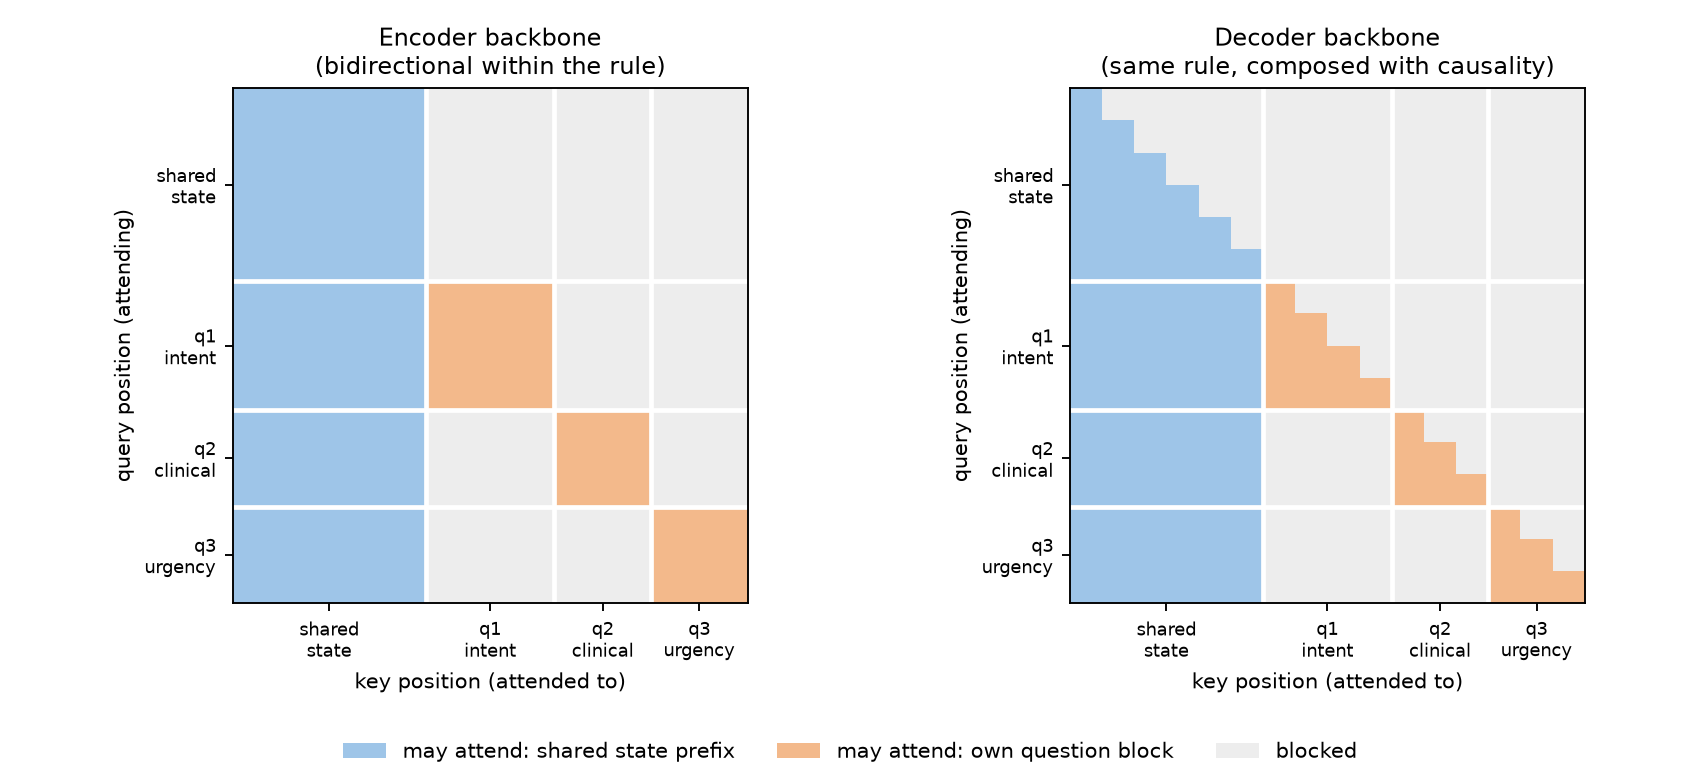
\includegraphics[width=\textwidth]{figures/attention_mask.png}
\caption{The mask of Eq.~\ref{eq:mask} for a packed sequence with a shared
state and three questions. Blue is attention to the shared prefix, orange
is attention within a question's own block, grey is blocked. No question
can see another, so its answer does not depend on what else was asked.
Right: the same rule composed with causality on a decoder backbone.}
\label{fig:mask}
\end{figure}

\paragraph{Memory.} The mask is $O(n^2)$ in sequence length, which is the
usual attention cost and not specific to this design, but it does bound
how many questions fit in one call. At our 2048-token budget a
ten-question router with 24 options packs comfortably; a 151-option menu
rendered with long descriptions does not, and the implementation degrades
by subsampling the menu (always keeping the gold) rather than failing.

\subsection{Readout and grouped normalisation}

Let $h_t$ be the final hidden state at marker position $t$, and let
$\mathcal{M}_i$ be the marker positions of question $q_i$. A scalar score
is produced per option. For an encoder backbone this is a shared linear
scorer, $z_t = w^\top h_t + b$. For a decoder backbone it is the difference
of two vocabulary logits at the marker,
\begin{equation}
  z_t = \big[W_{\text{lm}} h_t\big]_{\texttt{yes}} - \big[W_{\text{lm}}
  h_t\big]_{\texttt{no}},
  \label{eq:yesno}
\end{equation}
optionally plus a residual head $g(h_t)$ initialised to zero, so that
training begins at exactly the untrained readout.

Because $K_i$ differs across questions packed into one sequence, scores are
normalised \emph{within} each question rather than globally:
\begin{equation}
  p(o_{i,j}\mid s,q_i) = \frac{\exp(z_{t_{i,j}})}{\sum_{t\in\mathcal{M}_i}
  \exp(z_t)} .
  \label{eq:grouped}
\end{equation}
This is a segmented softmax over a ragged partition of the flat marker
array. Writing $y_i$ for the index of the gold option of question $q_i$,
and $\mathcal{A}$ for the questions this example actually answers (a row
may supervise only some of them), the loss is
\begin{equation}
  \mathcal{L} \;=\; -\frac{1}{|\mathcal{A}|}
  \sum_{i \in \mathcal{A}} \log p\big(o_{i,y_i} \mid s, q_i\big).
  \label{eq:loss}
\end{equation}

\paragraph{A worked example.} Suppose one packed sequence holds $q_1$ with
$K_1{=}3$ and $q_2$ with $K_2{=}2$, so the flat marker array has five
entries with scores $z = [2.0,\,1.0,\,0.5,\;\;0.2,\,1.4]$ and the
partition $\mathcal{M}_1 = \{1,2,3\}$, $\mathcal{M}_2 = \{4,5\}$. A global
softmax over all five would make $q_1$'s options compete with $q_2$'s,
which is meaningless. Grouped, we get $p_1 \approx [0.63, 0.23, 0.14]$ and
$p_2 \approx [0.23, 0.77]$, each summing to one. If the golds are
$y_1{=}1$ and $y_2{=}2$, then $\mathcal{L} = -\tfrac{1}{2}(\log 0.63 +
\log 0.77) \approx 0.36$.

\begin{algorithm}[t]
\caption{Forward pass for one packed instance}
\label{alg:forward}
\begin{algorithmic}[1]
\Require state $s$, questions $Q=\{q_i\}$ with option sets $O_i$
\State $x, b, \mathcal{M} \gets \textproc{Pack}(s, Q)$
  \Comment{tokens, block ids, marker positions}
\State $A \gets$ mask from Eq.~\ref{eq:mask} using $b$ and backbone
  constraint $C$
\State $H \gets \textproc{Backbone}(x, A)$
  \Comment{one forward pass, all questions}
\State $z \gets \textproc{Score}(H[\mathcal{M}])$
  \Comment{linear, or Eq.~\ref{eq:yesno} for a decoder}
\ForAll{questions $q_i$}
  \State $p_i \gets \textproc{Softmax}(z[\mathcal{M}_i])$
    \Comment{grouped, Eq.~\ref{eq:grouped}}
\EndFor
\State \Return $\{p_i\}$
\end{algorithmic}
\end{algorithm}

\subsection{Rendering the three primitives}

How an option is written to the sequence matters more than one would
expect, and \S\ref{sec:res-architecture} quantifies it. The rules we
converged on:

\begin{itemize}[leftmargin=1.4em,itemsep=0.25em]
  \item \choice{}: label and description both, since both carry meaning.
    Where the two are identical, as in multiple-choice tasks whose
    option \emph{is} its own description, they are collapsed, or every
    option is emitted twice.
  \item \score{}: the level description alone. Rendering a level as
    \texttt{"0: very negative: \ldots"} asks the model to score a bare
    index.
  \item \noul{}: bare polarity, \texttt{no}/\texttt{yes}, and \emph{not}
    the descriptions. A \noul{}'s two descriptions necessarily restate one
    judgement from opposite sides, so scoring both measures their overlap.
    Measured, this costs AUROC $0.63$ against $0.712$
    (\S\ref{sec:res-architecture}).
\end{itemize}

\subsection{Cost}

The state is encoded once regardless of $m$, so the marginal cost of a
question is its own options. Measured on the ten-question router with a
1.7B backbone, median latency per state is $69$\,ms for one question and
$74$\,ms for ten: \textbf{ten questions cost 6\% more than one}. The
reference API shows the same signature, $392$\,ms against $407$\,ms, which
is the evidence that it shares this design.

\paragraph{On the two sets of latency numbers in this paper.} The figures
here ($69$ and $74$\,ms) were taken while a training run shared the GPU;
those in \S\ref{sec:res-latency} ($37.7$ to $55.9$\,ms) were taken under
lighter load. Absolute values are therefore not comparable across the two
sections and only the within-section ratios are meaningful. We report both
rather than the flattering one, and neither is a throughput measurement:
everything here is batch size 1, which is the interactive case. Sustained
throughput under load is not measured in this work.

\section{Data}
\label{sec:data}

Since our central claim is that generalization lives in the training data
rather than the architecture, the data deserves the same scrutiny usually
reserved for the model.

\subsection{Training mixture}

We assemble 279 tasks and 323{,}466 rows from
\texttt{tasksource}~\cite{tasksource}, normalised into the typed-decision
format. Composition after cleaning:

\begin{center}
\begin{tabular}{lrl}
\toprule
primitive & tasks & notes \\
\midrule
\choice{} & 234 & option counts 2 to 174; 80 tasks have per-example menus \\
\noul{}   & 34  & \\
\score{}  & 11  & mostly three-level sentiment; see \S\ref{sec:discussion} \\
\midrule
total & 279 & 323{,}466 rows \\
\bottomrule
\end{tabular}
\end{center}

The lopsidedness is a limitation, not a design choice, and it predicts the
result pattern: \choice{} transfers best and \score{} worst.

\paragraph{Per-example option menus.} 80 tasks come from the
multiple-choice family, where each row carries its own answer set rather
than sharing a fixed menu. Supporting this in the trainer is what unlocked
that family, which is 261 of the 668 tasks \texttt{tasksource} exposes.

\subsection{Contamination guard}

A held-out suite is worthless if the training mixture contains the same
data under a different name, and aliasing is the normal case:
\texttt{tasksource} calls one dataset \texttt{banking77}, while the Hub
also carries \texttt{PolyAI/banking77} and \texttt{mteb/banking77}.

Each evaluation task therefore declares every alias of its source, a
manifest holds the union, and a matcher checks full names, owner-stripped
basenames, and glob patterns rather than performing a set intersection.
The check runs before every training run and refuses to proceed on a hit;
it excluded 23 tasks when building this mixture, and caught a real leak
during development. We verify it with a positive control --- injecting
\texttt{banking77} into a clean mixture and confirming rejection --- since
a guard that has never fired is indistinguishable from a guard that
cannot.

\subsection{Auditing, and what it found}
\label{sec:data-audit}

Training is the expensive step, so faults that survive it and surface
hours later as a bad number are worth catching first. We audit for gold
answers outside their own menu, \score{} golds stored as booleans (in
Python \texttt{True == 1}, which silently rewrites levels 0 and 1), class
imbalance too severe to learn, near-duplicate \noul{} descriptions, split
leakage, and contradictory labels.

Three findings changed the data materially.

\paragraph{The gold answer was always first.} \texttt{tasksource} ships
multiple-choice tasks correct-answer-first. Measured after ingestion, the
gold sat at index $0$ in \textbf{100\% of rows across all 83 ingested
tasks}. Stored that way, the data teaches ``pick the first option'' to
anything reading the menu as written. We shuffle at ingestion so the
stored data is honest, and drop tasks whose gold remains at a fixed index
or is a single constant string.

\paragraph{Contradictory labels.} 1{,}994 rows carried the same state under
the same menu with different answers; whichever the model predicts, some
are wrong, so the gradient is noise. One task contributed 195.

\paragraph{Menus too long to pack.} 1{,}787 rows had option sets exceeding
the context budget on their own, some options being multi-paragraph
passages.

Finally, we sweep every example through the same dataset object the
trainer uses, including augmentation, before training starts: 323{,}466
examples verified in 227 seconds of CPU. Two earlier runs died on packing
errors after twenty minutes and ten thousand steps respectively, and both
faults were findable in advance.

\subsection{Label-space augmentation}
\label{sec:data-aug}

Our mixture's option counts topped out near 20 while the evaluation suite
reaches 151. A model that has never seen a large menu collapses onto one
label when handed one, which is what an exact $0.000$ looks like: chance
alone would have produced roughly three correct in 200.

The intervention is to manufacture the missing shape. With probability
$\pi$, a training menu is padded with labels borrowed from other tasks in
the mixture, sampling a target size log-uniformly so small menus stay
common and large ones appear often enough to matter. The gold answer is
unchanged and still correct, so the example remains valid, but the model
must now discriminate against a large menu.

\begin{algorithm}[t]
\caption{Label-space augmentation for one \choice{} question}
\label{alg:aug}
\begin{algorithmic}[1]
\Require menu $O$ with gold $y$, distractor pool $D$, probability $\pi$,
  cap $M$
\If{$\textproc{Uniform}(0,1) \ge \pi$} \Return $O$ \EndIf
\State $n \gets \big\lfloor \exp\big(\textproc{Uniform}(\ln(|O|{+}1),\,
  \ln M)\big) \big\rfloor$ \Comment{log-uniform target size}
\State $E \gets \emptyset$
\While{$|O| + |E| < n$ and attempts remain}
  \State $d \sim D$
  \If{$d \notin O$ and $d \notin E$} \Comment{never add a plausibly correct label}
    \State $E \gets E \cup \{d\}$
  \EndIf
\EndWhile
\State \Return $\textproc{Shuffle}(O \cup E)$ \Comment{$y$ still present and correct}
\end{algorithmic}
\end{algorithm}

Option order is shuffled every epoch for a second reason: on the reference
system we measured the argmax flipping across option orderings on 7.5\% of
confusable items, at 2.8$\times$ the resampling floor. That is per-item
instability rather than a positional prior, so it cannot be corrected post
hoc and must be trained out.

\subsection{Evaluation suites}

\paragraph{Held-out suite (Study G).} Seven public tasks, 600 rows each,
never trained on: \texttt{clinc\_oos} ($K{=}151$), \texttt{banking77}
($K{=}77$), \texttt{massive\_intent} ($K{=}60$), \texttt{sst5} and
\texttt{helpsteer} (\score{}, $K{=}5$), \texttt{ag\_news} ($K{=}4$), and
\texttt{civil\_comments} (\noul{}). The high-cardinality end is the point:
a 151-way menu is where models that look fine on four-way classification
fail.

Every evaluation reports a \emph{held-in control}: accuracy on tasks the
model was trained on. If held-out is at chance and held-in is high, the
model genuinely fails to transfer; if both are at chance, it is a bug. We
also run a trivial three-way sanity task that any working harness must
pass. This is not ceremony --- the sanity check caught a real
partially-loaded-model bug that had produced a plausible, and wrong,
results table.

\paragraph{Healthcare router (Study S).} A synthetic pharmacy routing task:
988 items across 18 tiers, 395 train and 450 test, with ten questions per
item (one intent \choice{}, five topic \noul{}s, four safety gates).

Its first version was useless: the reference API scored a clean $1.000$ on
four of its tiers, which cannot distinguish any two systems. We rebuilt it
targeting where that system actually failed --- obliquely-worded clinical
risk, three-intent compounds, negation and conditionals, near-miss
out-of-scope, subtle prompt injection, and degraded voice-transcript text.
Splits are disjoint by content rather than by row, so paraphrases and
noisy variants of an item all stay in one split.

\section{Experimental setup}
\label{sec:experiments}

\subsection{Two studies}

The experiments answer two different questions, and they disagree. Keeping
them separate is what makes the disagreement legible rather than
contradictory.

\begin{description}[leftmargin=0em,itemsep=0.35em]
  \item[Study G (general capability).] Train on the 279-task mixture,
    evaluate on seven tasks never trained on. \emph{Does it work on a
    schema you have no labels for?} This is the harder claim and the
    reference system's main advantage.
  \item[Study S (specific use case).] Train on 395 examples of the
    healthcare router, evaluate on its 450-item test split. \emph{Given
    labels for your actual problem, how good does it get?}
\end{description}

\subsection{Backbones}

\begin{center}
\begin{tabular}{lll}
\toprule
 & encoder & decoder \\
\midrule
model & \texttt{ModernBERT-base} & \texttt{Qwen3-1.7B} \\
parameters & 150M & 1{,}725M \\
attention & bidirectional & causal + block-diagonal \\
readout & linear at marker & $\text{logit}(\texttt{yes}) - \text{logit}(\texttt{no})$ \\
\bottomrule
\end{tabular}
\end{center}

``Decoder'' names the attention pattern, not the usage: nothing is
generated token by token, and inference is a single forward pass with a
parallel read at marker positions.

\subsection{Training configurations}

Study G uses one epoch over the mixture, batch 16 (encoder) or 8
(decoder), context 2048, label-space augmentation at $\pi{=}0.5$ with cap
$M{=}120$. Study S uses six epochs over 395 examples. Four adaptation
regimes are compared in \S\ref{sec:res-router}: encoder full fine-tune,
decoder full fine-tune, decoder head-only, and decoder LoRA ($r{=}16$,
$\alpha{=}32$, on all attention and MLP projections, $\text{lr}=2\times
10^{-4}$).

\subsection{Metrics}

Accuracy, macro-F1, and multi-label exact-set match, with bootstrap
confidence intervals over examples. For comparability across tasks with
very different $K$ we report \emph{multiple of chance}, $\text{acc} \cdot
K$, since raw accuracy is not comparable: $0.28$ on a 77-way menu is
strong and on a 4-way menu is worse than guessing.

Two metric choices are load-bearing.

\paragraph{AUROC on binary tasks.} Argmax accuracy on a \noul{} describes
the $0.5$ threshold as much as the model. A task can rank almost perfectly
and still score exactly the class balance by putting all probability mass
on one side. We report both, and the gap between them is a calibration
result rather than a transfer result.

\paragraph{Chance is not always the right floor.} A skewed task can be
beaten by always predicting its most common label. Where that baseline
exceeds $1/K$ we test against it explicitly, which changes one of our
conclusions (\S\ref{sec:res-heldout}).

\paragraph{Paired comparison.} Against the reference system we use exact
McNemar on the same items, reporting $b_{10}$ (we are right, they are not)
and $b_{01}$. An aggregate delta cannot distinguish a real difference from
two systems disagreeing equally in both directions.

\subsection{Reproducibility}

All runs are on one H100. The contamination guard runs and logs on every
training run. Checkpoints record their backbone, adapter rank, prompt
preamble, option template, and fitted temperatures, because the same
weights scored under a different prompt are a different system. Artifacts
are listed in Appendix~\ref{app:artifacts}.

\section{Results}
\label{sec:results}

\subsection{The architecture does not generalize on its own}
\label{sec:res-architecture}

Before any task training, we score the held-out suite using only the
output format and a pretrained backbone.

\begin{center}
\begin{tabular}{llr}
\toprule
backbone & configuration & held-out mean \\
\midrule
encoder, 150M   & pretrained masked-LM head at the marker & 0.7$\times$ chance \\
encoder, 395M   & same readout, larger model              & 2.2$\times$ chance \\
\midrule
decoder, 1.7B   & state and options concatenated plainly  & 0.8$\times$ chance \\
decoder, 1.7B   & \quad + each option framed as yes/no    & 2.9$\times$ chance \\
decoder, 1.7B   & \quad + a preamble stating the task     & \textbf{11.5$\times$ chance} \\
decoder, 1.7B   & \quad \emph{control:} shortened framing & 5.7$\times$ chance \\
\bottomrule
\end{tabular}
\end{center}

The two halves of the table are different backbones and are not directly
comparable; each is internally consistent. Within the encoder rows, a
strong bidirectional model with a clever output format scores \emph{below
chance} and its larger sibling barely clears it. Within the decoder rows,
the format is worth an order of magnitude.

The last row is the control that matters: shortening the framing to
\texttt{\{opt\}\textbackslash ncorrect? answer} roughly halves the mean,
so the gain is the format doing work rather than an incidental wording
choice.

The same sensitivity appears in option rendering. On the held-out binary
task, scoring the two \noul{} descriptions rather than bare polarity costs
AUROC $0.63$ against $0.712$, because the descriptions restate one
judgement from opposite sides and a model scoring both measures their
overlap.

\subsection{Held-out transfer}
\label{sec:res-heldout}

Table~\ref{tab:heldout} gives the final encoder trained on the audited
279-task mixture. Harness sanity $1.000$; held-in control $1.1$--$2.3\times$.

\begin{table}[t]
\centering
\begin{tabular}{lrrrcr}
\toprule
task & $K$ & chance & accuracy & 95\% CI & $\times$ chance \\
\midrule
\texttt{clinc\_oos}      & 151 & 0.007 & 0.628 & [0.587, 0.672] & \textbf{94.9} \\
\texttt{massive\_intent} &  60 & 0.017 & 0.473 & [0.430, 0.512] & \textbf{28.4} \\
\texttt{banking77}       &  77 & 0.013 & 0.290 & [0.255, 0.323] & \textbf{22.3} \\
\texttt{ag\_news}        &   4 & 0.250 & 0.735 & [0.698, 0.772] & 2.9 \\
\texttt{sst5}            &   5 & 0.200 & 0.412 & [0.373, 0.452] & 2.1 \\
\texttt{civil\_comments} &   2 & 0.500 & 0.683 & [0.648, 0.718] & 1.4 \\
\texttt{helpsteer}       &   5 & 0.200 & 0.262 & [0.225, 0.297] & 1.3 \\
\midrule
\multicolumn{5}{l}{mean multiple of chance} & \textbf{21.9} \\
\bottomrule
\end{tabular}
\caption{Held-out transfer, 600 rows per task, never trained on. The suite
began this work at 0.9$\times$ chance. Every interval excludes its chance
floor.}
\label{tab:heldout}
\end{table}

\paragraph{One task is weaker than the table implies.} Against the
majority-class baseline rather than $1/K$, \texttt{civil\_comments} wins
outright ($0.683$ vs $0.500$, $p<10^{-15}$) but \texttt{helpsteer} sits on
the line: $0.262$ against a $0.233$ baseline, $p = 0.050$. Six of seven
are unambiguous; the seventh beats chance while only matching the trivial
baseline. The decoder of Section~\ref{sec:res-declora} removes this
caveat.

\subsection{A LoRA decoder transfers substantially better}
\label{sec:res-declora}

The same mixture, the same augmentation, rank-16 adapters on
Qwen3-1.7B instead of the encoder. This was the experiment our
pre-registered ablation plan named as deciding the architecture, and it
decides it clearly. Harness sanity $1.000$; held-in control
$1.5$--$2.5\times$, against the encoder's $1.1$--$2.3\times$.

\begin{table}[t]
\centering
\begin{tabular}{lrrcrr}
\toprule
task & $K$ & accuracy & 95\% CI & $\times$ chance & encoder \\
\midrule
\texttt{clinc\_oos}      & 151 & \textbf{0.783} & [0.752, 0.817] & \textbf{118.3} & 0.628 \\
\texttt{massive\_intent} &  60 & \textbf{0.773} & [0.738, 0.805] & \textbf{46.4}  & 0.473 \\
\texttt{banking77}       &  77 & \textbf{0.728} & [0.693, 0.765] & \textbf{56.1}  & 0.290 \\
\texttt{ag\_news}        &   4 & 0.803 & [0.772, 0.838] & 3.2  & 0.735 \\
\texttt{sst5}            &   5 & 0.438 & [0.400, 0.475] & 2.2  & 0.412 \\
\texttt{civil\_comments} &   2 & 0.688 & [0.655, 0.727] & 1.4  & 0.683 \\
\texttt{helpsteer}       &   5 & 0.282 & [0.247, 0.320] & 1.4  & 0.262 \\
\midrule
\multicolumn{4}{l}{mean multiple of chance} & \textbf{32.7} & 21.9 \\
\bottomrule
\end{tabular}
\caption{Held-out transfer, LoRA decoder against the encoder on identical
data and identical items. Every task improves.}
\label{tab:declora}
\end{table}

Two results matter here beyond the mean. First, \textbf{every task now
beats its majority-class baseline}, not merely $1/K$: \texttt{helpsteer}
reaches $0.282$ against $0.233$ at $p = 0.0025$, removing the single
caveat that qualified the encoder result. Second, \textbf{Banking77
zero-shot rises from $0.290$ to $0.728$} against the commercial
reference's $0.820$. A fifty-three point deficit becomes nine.

\paragraph{The architecture decision.} Our ablation registry fixed three
possible outcomes before this run so that the choice could not be
rationalised afterwards. Latency does not separate the backbones once the
adapter is merged ($1.07\times$, Section~\ref{sec:res-latency}), and a
1.7B model fits a consumer GPU, so zero-shot transfer was the deciding
axis. The decoder takes it by eleven multiples of chance. We therefore
recommend the LoRA decoder as the default artifact and retain the encoder
for deployments where p95 latency binds (20\,ms against 56\,ms) or where
a 0.6\,GB footprint outweighs nine points of zero-shot accuracy.

\begin{figure}[t]
\centering
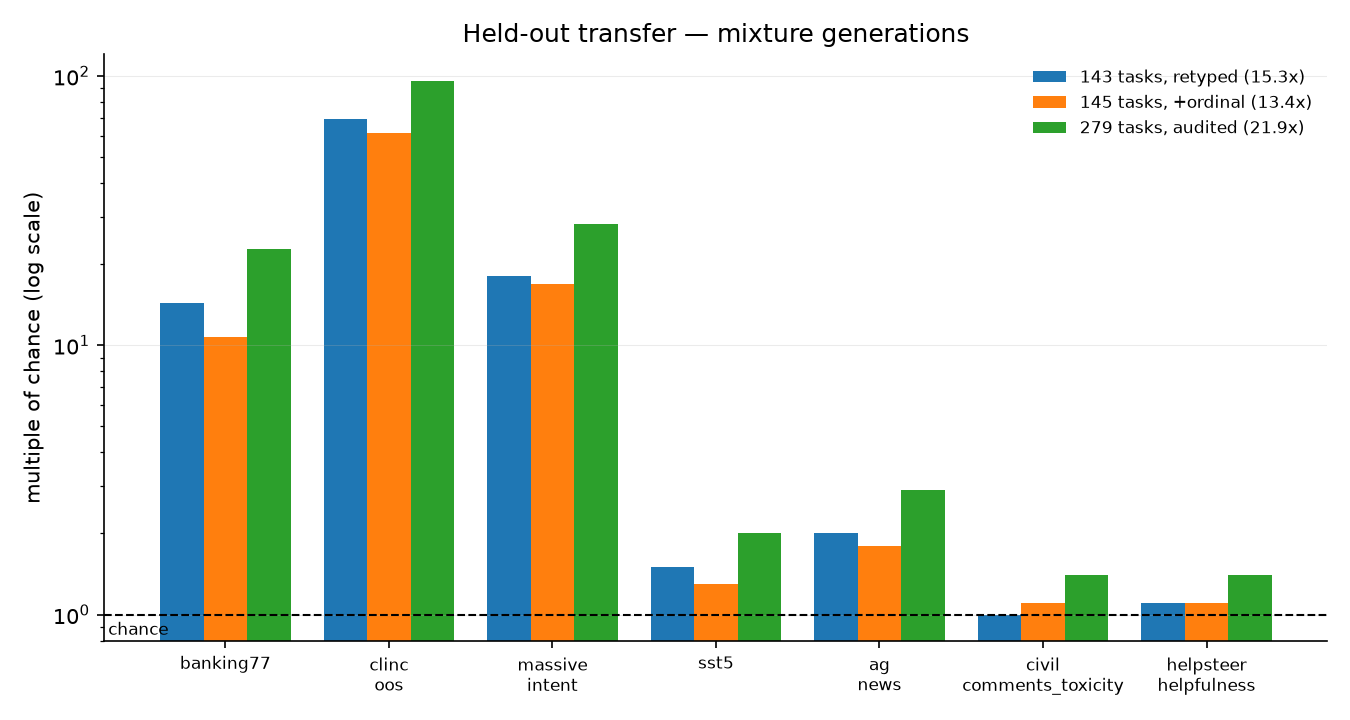
\includegraphics[width=0.95\textwidth]{figures/heldout_transfer.png}
\caption{Held-out transfer across three mixture generations, log scale,
chance marked. The middle generation is \emph{worse} than the first: that
is negative transfer from a mixture change that traded away \choice{}
tasks, retained here because a plot of only the best run would imply
progress that did not happen.}
\label{fig:transfer}
\end{figure}

\subsection{What produced the transfer}
\label{sec:res-data}

Label-space augmentation is the single largest effect we measured:

\begin{center}
\begin{tabular}{lrrr}
\toprule
held-out task & $K$ & before & after \\
\midrule
\texttt{banking77}       &  77 & 0.000 & \textbf{0.205} \\
\texttt{clinc\_oos}      & 151 & 0.000 & \textbf{0.180} \\
\texttt{massive\_intent} &  60 & 0.040 & \textbf{0.305} \\
\texttt{ag\_news}        &   4 & 0.225 & 0.655 \\
\bottomrule
\end{tabular}
\end{center}

Two exact zeroes become usable numbers. You do not need datasets with
large menus; you can synthesize them. The caveat is that the mixture also
grew from 61 to 141 tasks in the same change, so scale and shape are not
separated in this pair.

Scaling the audited mixture to 279 tasks took the mean from $17.6\times$
to $21.9\times$ and moved every task (Figure~\ref{fig:transfer}).

\subsection{Router: a fine-tuned small model against a zero-shot API}
\label{sec:res-router}

\paragraph{The comparison is asymmetric, in our favour, and we state it
before the numbers.} \openjev{} is fine-tuned on 395 labelled examples of
this task. The reference API is not: it has never seen this task's
training split, and produces its answers from the schema alone. This is
not a like-for-like contest, and a reader should discount it accordingly.
What it establishes is narrower than ``we beat Jev'': \emph{if you can
label a few hundred examples, a 1.7B open model reaches and passes a
closed API operating zero-shot on the same task.} That is a claim about
the value of labels as much as about either model.

\begin{table}[t]
\centering
\begin{tabular}{lrrrrrl}
\toprule
 & \openjev{} & reference & $b_{10}$ & $b_{01}$ & $p$ & winner \\
 & \emph{fine-tuned} & \emph{zero-shot} & & & & \\
\midrule
intent                        & \textbf{0.979} & 0.941 & 14 &  1 & 9.8e-04 & \openjev{} \\
multi-label exact set         & \textbf{0.909} & 0.822 & 57 & 18 & 7.2e-06 & \openjev{} \\
scope gate                    & \textbf{0.978} & 0.880 & 49 &  5 & 3.9e-10 & \openjev{} \\
clinical gate                 & 0.987 & 0.978 &  7 &  3 & 0.34 & level \\
abusive gate                  & 0.993 & 0.996 &  2 &  3 & 1.00 & level \\
injection gate                & 0.993 & 0.996 &  1 &  2 & 1.00 & level \\
\quad \texttt{compound\_3} tier & 0.903 & 0.645 & 11 &  3 & 0.057 & level \\
oblique clinical recall       & 0.966 & 0.793 &  5 &  0 & 0.063 & level \\
\bottomrule
\end{tabular}
\caption{Rank-16 LoRA on Qwen3-1.7B, 395 training examples, 258 seconds,
paired on the same 450 test items with exact McNemar. \openjev{} is
fine-tuned; the reference is zero-shot. Three wins, five ties, no losses.
The last two rows have $n{=}31$ and $n{=}29$, where even a large margin
struggles to reach significance: the oblique-clinical tier floors at
$p = 0.0625$ with zero losses.}
\label{tab:router}
\end{table}

\paragraph{Two rows that look like wins are not.} The
\texttt{compound\_3} tier ($0.903$ against $0.645$) and oblique clinical
recall ($0.966$ against $0.793$) are both large margins that fail the
significance test, at $p = 0.057$ and $p = 0.063$, because the tiers hold
31 and 29 items. We report them as level. They are the two tiers we most
expected to win, which is exactly why they need the test rather than the
margin.

\texttt{compound\_3} is nonetheless where the \noul{} primitive earns its
place in design terms: three simultaneous intents in one message, which a
single \choice{} softmax cannot express at all, whatever the $p$-value on
31 items says.

\paragraph{The smallest configuration is the best one.}

\begin{center}
\begin{tabular}{lrrr}
\toprule
configuration & intent & trainable & artifact \\
\midrule
encoder, all open            & 0.899 & 150M & 0.6 GB \\
decoder, head only           & 0.666 & 4.2M & 17 MB \\
decoder, all open            & 0.929 & 1{,}725M & 3.4 GB \\
\textbf{decoder, LoRA $r{=}16$} & \textbf{0.979} & \textbf{17M} & \textbf{87 MB} \\
\bottomrule
\end{tabular}
\end{center}

Adapting 17M parameters beats opening 1{,}725M, at $1/39$ the artifact.
The likely explanation is the learning rate a full fine-tune tolerates:
$10^{-5}$ over six epochs of 395 examples barely moves a 1.7B model, while
LoRA at $2\times10^{-4}$ adapts quickly without disturbing the weights it
rides on. Neither was tuned beyond one setting, so this is ``adapters are
the right default here'' rather than a tuned optimum.

\paragraph{Intermediate-task transfer.} Starting the encoder specialist
from a general checkpoint rather than raw weights, with identical data and
schedule, moves intent $0.544 \to 0.899$ and multi-label $0.453 \to 0.789$
($p = 6\mathrm{e}{-18}$). Two safety gates that never fired at all from
scratch reach $0.857$ and $0.583$ recall. This is the small-target-data
regime where STILTs predicts the largest gain.

\paragraph{But the general checkpoint was not needed here.} The $0.979$
LoRA used no mixture training at all; it started from base Qwen3-1.7B. The
general checkpoint earns its keep on schemas you have no labels for, not
on the task you actually care about.

\subsection{Latency}
\label{sec:res-latency}

\begin{center}
\begin{tabular}{lrrr}
\toprule
 & p50 & p95 & vs encoder \\
\midrule
encoder, 150M             & 37.7 ms & 50.9 ms & -- \\
decoder LoRA, unmerged    & 74.0 ms & 110.5 ms & 1.96$\times$ \\
decoder LoRA, merged      & \textbf{40.4 ms} & \textbf{55.9 ms} & \textbf{1.07$\times$} \\
\bottomrule
\end{tabular}
\end{center}

Measured back to back under identical load; read the ratios rather than
the absolute values. An unmerged adapter costs roughly $2\times$ for
nothing, since it is an extra matmul per target module at every layer.
Merged, a model eleven times larger runs 7\% slower.

\begin{figure}[t]
\centering
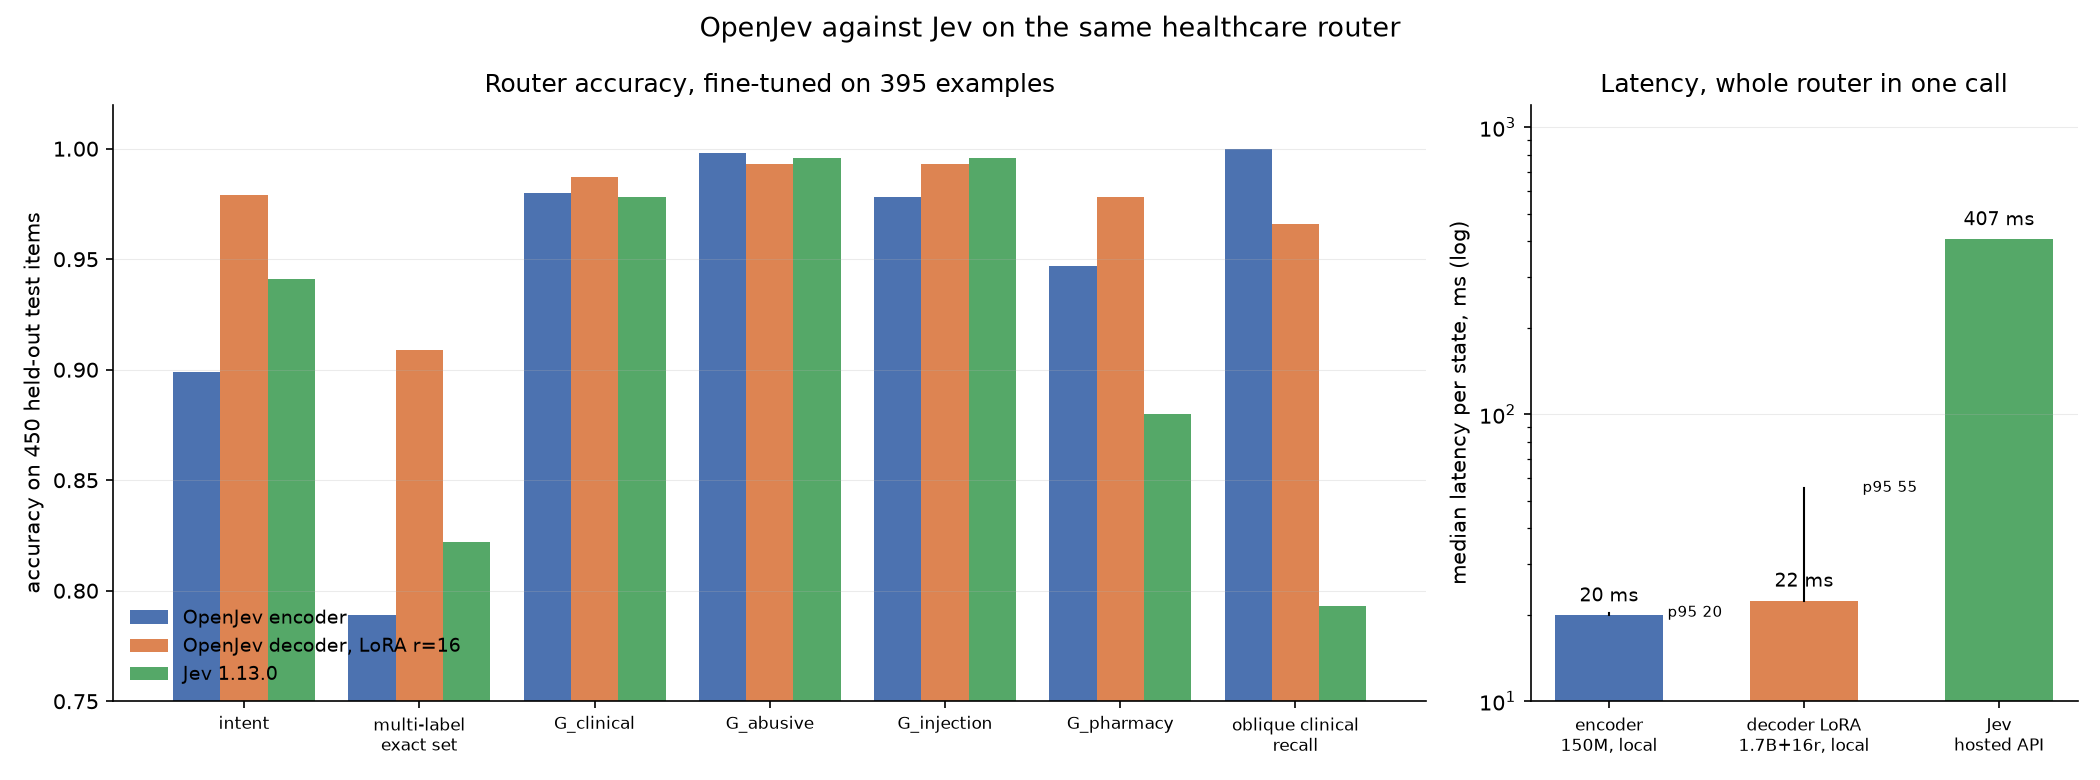
\includegraphics[width=\textwidth]{figures/comparison_router.png}
\caption{\openjev{} against the reference API on the router. Accuracy
left, latency right. The latency panel is not like-for-like: our figures
are local GPU compute and the reference is an end-to-end hosted call
including network, so it is the latency a user experiences rather than a
claim about their model's speed.}
\label{fig:comparison}
\end{figure}

\subsection{Benchmark transfer is not deployment readiness}
\label{sec:res-deployment}

The general checkpoint scores $21.9\times$ chance on the held-out suite.
Applied zero-shot to the routing task:

\begin{center}
\begin{tabular}{lrrr}
\toprule
 & zero-shot & fine-tuned & reference, zero-shot \\
\midrule
intent                & 0.601 & 0.902 & \textbf{0.941} \\
multi-label exact set & 0.427 & 0.789 & \textbf{0.822} \\
clinical gate recall  & \textbf{0.111} & 0.991 & 0.926 \\
\bottomrule
\end{tabular}
\end{center}

Intent at $0.601$ on a six-way menu is genuinely above chance, so the
transfer is real. It is also 34 points behind the reference, and the
clinical gate fires on one in nine of the cases it should catch, which is
not a gate. Clearing chance on academic benchmarks with clean label sets
is a materially weaker claim than working on a deployment task you have no
labels for, and the two come apart sharply here. Safety gates in
particular appear to require task supervision.

\section{Ablations, negative results, and one retraction}
\label{sec:ablations}

Reporting only what worked would misrepresent both the difficulty and the
method. This section holds the backbone we did not choose and the
evidence it produced, three interventions that sounded right and did
nothing or actively hurt, and one conclusion we published internally and
then withdrew.

\subsection{The encoder backbone: the alternative, and the control}
\label{sec:abl-encoder}

The bidirectional encoder was the first backbone we built and it is no
longer the recommended one. It is kept for two reasons. It is a released
artifact with a real deployment case (\S\ref{sec:when-backbone}), and it
is the control that makes several results in this paper legible: an
intervention that helps one backbone and hurts the other cannot be seen
with one backbone alone.

Table~\ref{tab:heldout-enc} is the encoder trained on the same audited
279-task mixture, with the same augmentation, evaluated on the same items
at full menu size. Harness sanity $1.000$; held-in control $1.1$ to
$2.3\times$ chance.

\begin{table}[t]
\centering
\begin{tabular}{lrrrcr}
\toprule
task & $K$ & chance & accuracy & 95\% CI & $\times$ chance \\
\midrule
\texttt{clinc\_oos}      & 151 & 0.007 & 0.382 & [0.342, 0.420] & \textbf{57.6} \\
\texttt{massive\_intent} &  60 & 0.017 & 0.473 & [0.430, 0.512] & \textbf{28.4} \\
\texttt{banking77}       &  77 & 0.013 & 0.343 & [0.305, 0.382] & \textbf{26.4} \\
\texttt{ag\_news}        &   4 & 0.250 & 0.735 & [0.698, 0.772] & 2.9 \\
\texttt{sst5}            &   5 & 0.200 & 0.412 & [0.373, 0.452] & 2.1 \\
\texttt{civil\_comments} &   2 & 0.500 & 0.683 & [0.648, 0.718] & 1.4 \\
\texttt{helpsteer}       &   5 & 0.200 & 0.262 & [0.225, 0.297] & 1.3 \\
\midrule
\multicolumn{5}{l}{mean multiple of chance} & \textbf{17.2} \\
\bottomrule
\end{tabular}
\caption{Held-out transfer for the encoder, 600 rows per task, never
trained on, every task scored at its full advertised menu. This is the
comparison column of Table~\ref{tab:heldout} in full. Every interval
excludes its chance floor, and the suite began this work at 0.9$\times$
chance. An earlier draft reported $21.9\times$ here from an in-training
evaluator run against a superseded version of the suite; these figures
come from \texttt{eval\_heldout.py} on the published checkpoint and the
published suite, and reproduce from a clean clone.}
\label{tab:heldout-enc}
\end{table}

This is a real result and we do not withdraw it: all seven tasks clear
their chance floor and a 151-way menu reaches $57.6\times$. It is also
the weaker of the two backbones on every task, and one task is weaker
than the table implies. Against the majority-class baseline rather than
$1/K$, \texttt{civil\_comments} wins outright ($0.683$ against $0.500$,
$p<10^{-15}$) but \texttt{helpsteer} sits on the line: $0.262$ against a
$0.233$ baseline, $p = 0.050$. Six of seven are unambiguous; the seventh
beats chance while only matching the trivial baseline. The decoder
removes that caveat, though its own \texttt{helpsteer} margin is thin
($p = 0.010$).

\paragraph{Three findings the encoder is responsible for.} None of these
survives if you only ever train one backbone.

\begin{itemize}[leftmargin=1.4em,itemsep=0.3em]
  \item \textbf{The output format confers nothing by itself.} Untrained,
    with the option-scoring readout and no task training, the encoder
    scores $0.7\times$ chance, worse than guessing, and its 395M sibling
    reaches $2.2\times$ (\S\ref{sec:res-architecture}). An untrained
    decoder reads menus at $11.5\times$, but only because it borrows a
    pretrained vocabulary head, which is a property of the backbone and
    not of the architecture. The encoder is what separates those two
    explanations.
  \item \textbf{Intermediate-task transfer reverses by backbone.}
    $+36$ points on the encoder and significantly negative on the
    decoder, from the identical intervention (\S\ref{sec:abl-sd6}).
  \item \textbf{Benchmark transfer does not rank models on deployment.}
    The decoder beats the encoder on all seven public tasks and is worse
    than it zero-shot on the router (\S\ref{sec:res-deployment}). With
    one backbone this would have read as a flat statement that zero-shot
    routing is hard, rather than as a reversal.
\end{itemize}

\subsection{Interventions that failed}

\paragraph{Ordinal scale augmentation: null.}
The mixture's \score{} tasks are mostly three-level sentiment scales,
against a held-out task wanting a five-level judgement. We synthesized the
missing diversity the way label-space augmentation synthesized menu size:
merging adjacent levels and remapping the gold, and restating a scale in
another vocabulary of the same length within its semantic family. Ablated
at $\pi_{\text{scale}} \in \{0, 0.5\}$ with everything else fixed:

\begin{center}
\begin{tabular}{lrr}
\toprule
 & $\pi_{\text{scale}}{=}0$ & $\pi_{\text{scale}}{=}0.5$ \\
\midrule
\texttt{helpsteer} & 0.110 (0.6$\times$) & 0.128 (0.6$\times$) \\
\texttt{sst5}      & 0.342 (1.7$\times$) & 0.348 (1.7$\times$) \\
suite mean         & \textbf{16.5$\times$} & 15.7$\times$ \\
\bottomrule
\end{tabular}
\end{center}

Both ordinal tasks land on the same multiple of chance either way, and the
mean is slightly \emph{worse} with it. The mechanism is correct and tested
(golds stay on the right level, merges stay contiguous and monotone)
it simply is not the bottleneck.

\paragraph{Adding a primitive by removing another: negative, twice.}
The mixture was poor in \noul{} (13 tasks) and \score{}. We recovered 21
real yes/no tasks by recognising negation pairs (\texttt{not\_paraphrase}
vs \texttt{paraphrase}) that the builder had been emitting as two-option
menus, and separately added two real ordinal datasets. Both made things
worse:

\begin{center}
\begin{tabular}{lrrr}
\toprule
mixture & \choice{} tasks & \texttt{banking77} & suite mean \\
\midrule
143 tasks, baseline          & 121 & 0.278 & \textbf{17.6$\times$} \\
143 tasks, 21 retyped to \noul{} & 100 & 0.187 & 15.3$\times$ \\
145 tasks, + 2 ordinal       & 100 & 0.138 & 13.4$\times$ \\
\bottomrule
\end{tabular}
\end{center}

\texttt{banking77} tracks the \choice{} task count exactly. Five of seven
held-out tasks are \choice{}, so converting or diluting \choice{} tasks is
a trade rather than an improvement. This is textbook negative
transfer~\cite{stilts}, and we caused it twice before measuring it. The
fix was scale: the audited 279-task mixture restored \choice{} to 234 and
added tasks on top, reaching $17.2\times$.

\subsection{A conclusion we retracted}

For several runs we reported that the \noul{} primitive does not transfer,
on the evidence that the held-out binary task sat at exactly $0.500$
accuracy with macro-F1 $0.333$, which is a model answering the same way every
time. We spent two separate interventions on it.

Both were aimed at the wrong thing. The model ranks that task at AUROC
$0.714$ and reaches $0.680$ accuracy at a fitted threshold; it puts 98\% of
its probability mass above $0.5$, so argmax calls everything positive and
accuracy lands on the class balance. \textbf{That is a calibration result,
not a transfer result.} Reporting argmax accuracy alone on an uncalibrated
binary measures the threshold as much as the model, and our evaluation now
reports AUROC alongside it.

Two measurement errors of our own contributed, and both are worth stating
because they are easy to repeat:

\begin{itemize}[leftmargin=1.4em,itemsep=0.3em]
  \item \textbf{A label inversion in the inference helper.} Option names
    were derived in \emph{dictionary} order, so a \noul{} whose criteria
    were written \texttt{\{true: \ldots, false: \ldots\}} had its two
    probabilities swapped. This turned AUROC $0.712$ into $0.288$,
    exactly $1 - 0.712$, and looked like a model ranking toxic comments
    as cleaner than clean ones. The giveaway was the arithmetic.
  \item \textbf{A partially loaded model that produced a full results
    table.} A decoder was built without its trained head, so
    \texttt{load\_state\_dict(strict=False)} silently dropped six tensors
    and scored the untrained readout, reporting $5.8\times$ chance where
    the truth was $16.2\times$. A warning printed; a complete results table
    printed under it. Loaders now raise.
\end{itemize}

We also credited the held-in control with catching the second bug, and
that was wrong too: the decoder reads $1.0$ to $1.3\times$ on held-in tasks
even when it loads perfectly, because a 4.2M head on a frozen backbone
barely fits its own training mixture. Only the harness sanity task caught
it.

\subsection{Intermediate-task transfer helps the encoder and hurts the
decoder}
\label{sec:abl-sd6}

The clearest illustration that an intervention is not good in itself, only
good relative to what the base model already does. Initialising the
router adapter from the general adapter of \S\ref{sec:res-heldout},
rather than from base Qwen3, and training identically:

\begin{center}
\begin{tabular}{lcc}
\toprule
initialisation & intent accuracy & 95\% CI \\
\midrule
base Qwen3          & \textbf{0.979} & [0.962, 0.994] \\
general adapter     & 0.953 & [0.926, 0.973] \\
\bottomrule
\end{tabular}
\end{center}

Paired McNemar on the same 338 items: $p = 0.012$, with 10 items the
base initialisation gets right that the general one misses against 1 in
the other direction. The general initialisation is significantly
\emph{worse}.

On the encoder path the identical intervention was worth $+36$ points.
The contradiction resolves on what each backbone lacked. The encoder had
to learn the very notion of scoring against a menu from 395 router
examples, so the mixture supplied a missing capability. Base Qwen3
already reads menus from pretraining, so the mixture supplies nothing new
and its 279-task specialisation acts as interference on a narrow
fourteen-intent problem. This is negative transfer, the second instance
measured in this work.

The practical rule we draw: stage your fine-tuning when the base model
cannot perform the task \emph{form} at all, and train the task adapter
directly from base once it can. The general adapter remains the right
artifact for zero-shot use, where by definition no task data exists to
train on; it is the wrong starting point when task data does exist.

\subsection{Interventions that worked}

For completeness, the positive results, ordered by effect size: label-space
augmentation (\S\ref{sec:res-data}); the decoder backbone over the encoder
($17.2\times \to 29.6\times$, \S\ref{sec:res-heldout}); mixture scale and
auditing ($17.6\times \to 17.2\times$); prompt format on a decoder backbone
($0.8\times \to 11.5\times$); intermediate-task transfer on the encoder
only ($+36$ points at 395 target examples, and see
\S\ref{sec:abl-sd6} for where it reverses); LoRA over full fine-tuning
($0.979$ vs $0.929$ at $1/39$ the size); and adapter merging
($1.96\times \to 1.07\times$ latency).

\subsection{Methodological caveat}

One choice in this paper was made badly. The \noul{} rendering rule
(\S\ref{sec:method}) was selected by comparing variants on the held-out
task itself, which is the wrong place to choose anything. The change is
principled and small, and the three-way spread we observed across
connective phrasings ($0.25$ to $0.75$ AUROC) is large enough that it
should be re-settled on held-in data before the held-out number is quoted
as clean.

\section{Discussion}
\label{sec:discussion}

\subsection{What the evidence supports}

The split is clean and it is about labels. \textbf{Given roughly 400
labelled examples for your task, a 1.7B model with an 87\,MB adapter beats
a commercial typed-decision API} on a hardened routing benchmark, runs on
your own hardware, returns full-precision probabilities, and is
deterministic. \textbf{Without labels, it does not come close}: $0.290$ on
Banking77 against roughly $0.820$.

Both halves matter. The first says the capability is not gated behind
scale or a vendor. The second says the vendor's actual product --- working
on a schema you have never labelled --- is a real and unsolved thing.

\subsection{Why the data mattered more than the model}

The most useful finding here is negative: a strong encoder with a clever
output format scores below chance untrained. Nothing about scoring options
at marker positions confers generalization. What produced it was the
composition of the training mixture, and in particular a property we could
manufacture --- menu-size diversity --- rather than one we had to find.

This has a practical consequence. Our mixture is 234 \choice{} tasks
against 34 \noul{} and 11 \score{}, and the result pattern follows exactly:
\choice{} transfers, the other two barely do. That is a statement about
279 tasks scraped from one source, not about the architecture. The
fastest route to a better general model is a more balanced typed-decision
corpus, and assembling one is beyond what a single project can do.

\subsection{Limitations}

\paragraph{The ordinal primitive is weak.} \texttt{helpsteer} beats chance
but only draws level with predicting the most common label. The mixture
has 11 \score{} tasks, mostly three-level sentiment. We searched twice for
more; ordinal scales with five or more levels, in domains that are not
response quality, are scarce in accessible form. We deliberately excluded
LLM-response-rating corpora because they are the held-out task in all but
name, and training on a near-twin would move the number without moving the
ability.

\paragraph{No ordinal or rejection head.} \score{} is a softmax over
levels; we use the ordering only in rendering and in an expectation-based
readout. Rank-consistent objectives~\cite{corn} and adaptive rejection
boundaries~\cite{adb} are the obvious next step and are not implemented.

\paragraph{Zero-shot on a real task is much worse than on benchmarks.}
$21.9\times$ chance on the held-out suite coexists with intent $0.601$ and
a clinical-gate recall of $0.111$ on the routing task. Safety gates in
particular appear to need task supervision, and we would not deploy any
zero-shot gate on this evidence.

\paragraph{Synthetic evaluation.} The routing task is handwritten and
systematically composed, not real traffic. It is evidence a method works,
not a claim about any production distribution.

\paragraph{One-day black-box baseline.} All reference figures are
measurements of a hosted endpoint on a single day from one network
location.

\paragraph{Untuned comparisons.} The LoRA-versus-full-fine-tune result
compares one hyperparameter setting each. We believe the direction and
not the magnitude.

\subsection{Future work}

The experiment that would most change these conclusions is a balanced
typed-decision corpus with real \score{} and \noul{} diversity at the
scale Flan suggests. Beyond that: adapter composition, where a task
adapter is initialised from a general adapter, which is the
parameter-efficient analogue of the $+36$-point intermediate-task result;
rank-consistent ordinal heads; and calibrated rejection for out-of-scope
inputs.

\subsection{Conclusion}

Typed decisions do not need a large model, and they do not need
generation. They need the right output format, an attention mask that
keeps questions independent, and --- overwhelmingly --- training data
whose \emph{shape} matches deployment. Of those three, only the last was
hard, and it is the one that transfers least from the literature to
practice.



\bibliographystyle{plain}
\bibliography{refs}

\appendix
\section{Terminology for readers new to the area}
\label{app:glossary}

This appendix defines every term the paper uses, assuming no background.
Nothing here is needed by a reader who already works on language models;
it exists so the main text can stay short.

\subsection{The problem}

\begin{description}[leftmargin=0em,style=nextline,itemsep=0.3em]

\item[State] The input being judged: a customer message, a product review,
a comment. One state can have many questions asked about it.

\item[Question] One decision to make about the state, with instructions
and a set of candidate answers.

\item[Option, menu, criteria] Used interchangeably for the candidate
answers of a question. A \emph{fixed menu} is shared by every row of a
task; a \emph{per-example menu} differs row by row, as in reading
comprehension where each question has its own answers.

\item[$K$] The number of options. $K{=}151$ means a 151-way choice.

\item[Primitive] The type of a question: \choice{} (pick one of $K$),
\score{} (pick one level on an ordered scale), \noul{} (yes or no).

\item[Multi-label] When more than one label can be true at once. A single
\choice{} cannot express this, because its probabilities sum to one across
options. Several \noul{} questions can.

\end{description}

\subsection{How models process text}

\begin{description}[leftmargin=0em,style=nextline,itemsep=0.3em]

\item[Token] A chunk of text, roughly a word piece. Models read and write
sequences of tokens, not characters.

\item[Embedding, hidden state] The vector a model holds for each token
position after processing. The hidden state at a position is what we read
a decision from.

\item[Attention] The mechanism by which a token's representation is built
from other tokens. An \emph{attention mask} says which positions may look
at which.

\item[Encoder vs decoder] Two attention patterns. An \textbf{encoder} is
bidirectional: every token sees every other. A \textbf{decoder} is causal:
a token sees only what came before it, which is what makes text generation
possible. \textbf{In this paper ``decoder'' names the attention pattern
only.} We never generate text; we run one forward pass and read scores.
The decoder is the backbone we recommend; the encoder is the documented
alternative (\S\ref{sec:when-backbone}).

\item[Forward pass] One run of the model over an input. Our central
efficiency claim is that $m$ questions cost one forward pass, not $m$.

\item[Logit] A raw, unnormalised score. Logits become probabilities
through a softmax.

\item[Softmax] Turns a vector of logits into probabilities that sum to
one. Our \emph{grouped} softmax does this separately within each
question's options, because questions in one packed sequence have
different $K$.

\item[Backbone] The pretrained model we build on, before any of our
training.

\end{description}

\subsection{Training}

\begin{description}[leftmargin=0em,style=nextline,itemsep=0.3em]

\item[Pretraining] The expensive first stage, done by others, where a
model learns language from large text corpora. We never do this.

\item[Fine-tuning] Further training of a pretrained model on a specific
task. Cheap by comparison: 38 seconds in one of our settings.

\item[Epoch] One pass over the training data.

\item[Learning rate] How large a step training takes per update. It
matters more than it sounds: our LoRA-beats-full-fine-tuning result is
most likely a learning-rate effect (\S\ref{sec:res-router}).

\item[Frozen] A parameter that is not updated during training.

\item[LoRA (Low-Rank Adaptation)] Instead of updating a large weight
matrix, train two small matrices alongside it and add their product. The
large matrix stays frozen. The \textbf{rank} $r$ sets how small; $r{=}16$
here. The result is an \textbf{adapter} of tens of megabytes rather than
gigabytes, so one backbone can serve many tasks.

\item[Merging] Folding a trained adapter back into the frozen weights, so
inference costs no extra work. An unmerged adapter is roughly twice as
slow for no benefit (\S\ref{sec:res-latency}).

\item[Multi-task mixture] Training on many tasks at once, so the model
learns the general shape of the problem rather than one instance of it.

\item[Intermediate-task transfer] Train on task A, then on target task B.
Helps most when B is small. Known in the literature as
STILTs~\cite{stilts}.

\item[Negative transfer] When adding training data makes the target
\emph{worse}. We caused this twice (\S\ref{sec:ablations}).

\end{description}

\subsection{Evaluation}

\begin{description}[leftmargin=0em,style=nextline,itemsep=0.3em]

\item[Zero-shot] Evaluating on a task the model was never trained on. The
hard claim, and the thing Jev is good at.

\item[Held-out] Data deliberately excluded from training, used to measure
zero-shot ability. Worthless if it leaks into training, hence the
contamination guard.

\item[Held-in control] Accuracy on tasks the model \emph{was} trained on,
reported next to held-out. If held-out is at chance and held-in is high,
the model truly fails to transfer; if both are at chance, something is
broken. Without this, a bug and a finding look identical.

\item[Chance] What random guessing scores: $1/K$. On a 151-way menu that
is $0.007$, so an accuracy of $0.29$ is strong; on a 4-way menu chance is
$0.25$ and $0.29$ is nearly worthless.

\item[Multiple of chance] Accuracy divided by chance, so tasks with very
different $K$ can be compared on one axis.

\item[Majority-class baseline] Always predicting the most common label.
On skewed data this beats chance, so it is the stricter floor. One of our
encoder results passes the chance test and only ties this one
(\S\ref{sec:abl-encoder}).

\item[Accuracy, precision, recall] Accuracy is the fraction correct.
\emph{Recall} is the fraction of true positives found, which is what
matters for a safety gate. \emph{Precision} is the fraction of positive
predictions that were right.

\item[Macro-F1] The harmonic mean of precision and recall, averaged over
classes so rare classes count as much as common ones. A binary task
scoring macro-F1 $0.333$ is predicting one class for everything.

\item[AUROC] Ranking quality, independent of any threshold: the
probability a random positive is scored above a random negative. $0.5$ is
chance. It matters because a model can rank well and still score badly at
a fixed threshold, which is a calibration problem and not a capability
one.

\item[Calibration] Whether a stated probability matches reality. If
everything a model calls $0.7$ is right $70\%$ of the time, it is
calibrated. \textbf{ECE} measures the gap; \textbf{temperature scaling} is
the standard post-hoc fix.

\item[Bootstrap confidence interval] Resample the test set with
replacement many times and report the middle 95\% of the resulting scores.
An interval that excludes chance means the result is unlikely to be luck.

\item[McNemar test] For comparing two systems on the \emph{same} items.
Counts only the disagreements: $b_{10}$ where we are right and they are
not, $b_{01}$ the reverse, and asks whether the split is lopsided enough
to be real. Necessary because two systems can have equal accuracy while
disagreeing on a third of the set.

\item[$p$-value] Informally, the probability of seeing a difference this
large if there were no real difference. Below $0.05$ is conventionally
called significant. With small samples, significance can be unreachable
no matter how good the model: one of our tiers has 29 items, so even a
perfect score floors at $p = 0.0625$.

\end{description}

\subsection{Terms specific to this work}

\begin{description}[leftmargin=0em,style=nextline,itemsep=0.3em]

\item[Packing] Writing the state once, then all questions and options
after it, as one sequence for one forward pass.

\item[Shared prefix] The state portion of a packed sequence, attended to
by every question. The reason $m$ questions are nearly free.

\item[Marker] A token after each option where its score is read.

\item[Block-diagonal attention] The mask that lets each question see the
shared prefix and itself, but not other questions, so an answer does not
depend on what else was asked.

\item[Label-space augmentation] Padding a training menu with labels
borrowed from other tasks. The gold stays correct, but the model must
discriminate against a larger menu. Our largest single effect.

\item[Distractor] One of those borrowed labels.

\item[Contamination guard] A check that no evaluation dataset appears in
the training mixture under any of its names.

\end{description}

\section{Released artifacts}
\label{app:artifacts}

All public and Apache 2.0 unless the underlying data says otherwise.

\paragraph{Code.} \url{https://github.com/S1LV3RJ1NX/openjev}

\paragraph{Models.}
\begin{center}
\small
\begin{tabular}{lll}
\toprule
artifact & size & identifier \\
\midrule
General encoder checkpoint & 0.6 GB & \texttt{s1lv3rj1nx/openjev-encoder-general} \\
Router LoRA adapter & 87 MB & \texttt{s1lv3rj1nx/openjev-router-lora} \\
Router encoder specialist & 0.6 GB & \texttt{s1lv3rj1nx/openjev-router-healthcare} \\
\bottomrule
\end{tabular}
\end{center}

\paragraph{Datasets.}
\begin{center}
\small
\begin{tabular}{lll}
\toprule
artifact & size & identifier \\
\midrule
Training mixture & 279 tasks / 323{,}466 rows & \texttt{s1lv3rj1nx/openjev-mixture} \\
Held-out suite & 7 tasks / 4{,}200 rows & \texttt{s1lv3rj1nx/openjev-heldout} \\
Healthcare router & 988 items / 18 tiers & \texttt{s1lv3rj1nx/openjev-healthcare-router} \\
\bottomrule
\end{tabular}
\end{center}

Base models: \texttt{answerdotai/ModernBERT-base}~\cite{modernbert} and
\texttt{Qwen/Qwen3-1.7B}~\cite{qwen3}.

\section{Reproducing the main results}
\label{app:repro}

\begin{center}
\small
\begin{tabular}{ll}
\toprule
result & command \\
\midrule
Held-out transfer & \texttt{scripts/eval\_heldout.py --ckpt <ckpt>} \\
Router against reference & \texttt{scripts/eval\_router.py --ckpt <ckpt> --dump o.json} \\
Paired McNemar & \texttt{scripts/compare\_to\_jev.py --ours o.json --jev j.json} \\
Latency & \texttt{scripts/bench\_latency.py --ckpt <ckpt>} \\
Data audit & \texttt{scripts/audit\_data.py <task dir> --deep} \\
Packing check & \texttt{scripts/check\_packing.py <mixture>} \\
Binary diagnosis & \texttt{scripts/diagnose\_binary.py --ckpt <ckpt>} \\
\bottomrule
\end{tabular}
\end{center}

\section{Hyperparameters}
\label{app:hparams}

\begin{center}
\small
\begin{tabular}{lll}
\toprule
 & Study G (mixture) & Study S (router) \\
\midrule
epochs & 1 & 6 \\
batch size & 16 enc / 8 dec & 8 enc / 4 dec \\
context & 2048 & 2048 enc / 3072 dec \\
learning rate & $3\times10^{-5}$ enc & $3\times10^{-5}$ enc, $2\times10^{-4}$ LoRA \\
label-space aug. $\pi$ & 0.5, cap 120 & off \\
\noul{} recast $\pi$ & 0.15 & off \\
LoRA & $r{=}16$, $\alpha{=}32$, dropout 0.05 & same \\
LoRA targets & \multicolumn{2}{l}{\texttt{q,k,v,o,gate,up,down} projections} \\
\bottomrule
\end{tabular}
\end{center}

Temperature scaling is fitted on a dev split after training and stored
with the checkpoint.

\section{Held-out suite composition}
\label{app:suite}

\begin{center}
\small
\begin{tabular}{llrl}
\toprule
task & primitive & $K$ & source \\
\midrule
\texttt{clinc\_oos} & \choice{} & 151 & \texttt{clinc/clinc\_oos} \\
\texttt{banking77} & \choice{} & 77 & \texttt{PolyAI/banking77} \\
\texttt{massive\_intent} & \choice{} & 60 & \texttt{AmazonScience/massive} \\
\texttt{ag\_news} & \choice{} & 4 & \texttt{fancyzhx/ag\_news} \\
\texttt{sst5} & \score{} & 5 & \texttt{SetFit/sst5} \\
\texttt{helpsteer\_helpfulness} & \score{} & 5 & \texttt{nvidia/HelpSteer} \\
\texttt{civil\_comments\_toxicity} & \noul{} & 2 & \texttt{google/civil\_comments} \\
\bottomrule
\end{tabular}
\end{center}

Each task declares every alias of its source; the union is the
contamination manifest checked before every training run.


\end{document}
